\documentclass{beamer}

\usepackage{beamerthemevictor,comment,verbatim,graphicx,rotating}

\newcommand{\TbT}{\TeX\ by Topic}
\newcommand{\Metafont}{\textsc{Metafont}}
\let\metafont\Metafont
\newcommand\ascii{{\sc Ascii}}
\newcommand\ebcdic{{\sc Ebcdic}}
\newcommand\gnuplot{\protect\n{gnuplot}}
\def\mod{\mathbin{\mathrm{mod}}}
\def\eqref#1{equation~(\ref{#1})}
\def\Eqref#1{Equation~(\ref{#1})}
\def\inv{^{-1}}
\def\endproof{\unskip\penalty10000 \hskip10pt plus 1fill$\bullet$\par}

\def\etal{\textit{et al.}}
\def\lex{{\it lex}}
\def\yacc{{\it yacc}}
\def\make{{\it make}}
\def\web{{\textsc{Web}}}
\def\n{\bgroup
  \catcode`\#=12 \catcode`\_=12 \catcode`\^=12
  \catcode`\&=12 
  \tt \let\next=}
\newcommand{\cs}[1]{{\tt\char`\\#1}}
{\catcode`\.=13
 \gdef.{${}_\bullet$}
}
\def\parserule#1{%
    \ifmmode \n{#1}\,\rightarrow\relax
    \else $\n{#1}\,\rightarrow{}$\nobreak
    \fi
    \hbox\bgroup\catcode`\.=13 \tt\let\next=}

\newenvironment{remark}%
    {\medskip\noindent{\bf Remark.}}{}
\usepackage{bnf}
\input bnf.env

\generalcomment{inputwithcode}
  {\begingroup\def\ProcessCutFile{}}
  {\verbatiminput{\CommentCutFile}
   \endgroup
   \input{\CommentCutFile}
  }
\generalcomment{examplewithcode}
  {\begingroup
     \def\ProcessCutFile{}\def\CommentCutFile{example.tex}}
  {\verbatiminput{\CommentCutFile}
   Output:
   \begin{quote}
     \begin{minipage}[t]{3in}
        \everypar{}
        \input{\CommentCutFile} 
     \end{minipage}
   \end{quote}
   \endgroup
  }
\specialcomment{ttexamplewithcode}
  {\begingroup\def\ProcessCutFile{}}
  {\verbatiminput{\CommentCutFile}
   \endgroup
   Output:
   \begin{quote}\begin{ttfamily} \input{\CommentCutFile} 
     \end{ttfamily}\end{quote}
  }
\generalcomment{mathexamplewithcode}
  {\begingroup\def\ProcessCutFile{}}
  {\verbatiminput{\CommentCutFile}
   Output:
   \begin{equation} \input{\CommentCutFile} \end{equation}
   \endgroup
  }

\def\chaptertitle{\csname\chaptername title\endcsname}
\def\chaptershorttitle{\csname\chaptername shorttitle\endcsname}

\def\lambdatitle{Lambda calculus in \TeX}
\def\lambdashorttitle{Lambda calculus}

\def\latextitle{Yet another \LaTeX\ tutorial}
\def\latexshorttitle{\LaTeX}

\def\lextitle{A \lex\ tutorial}
\def\lexshorttitle{\lex}

\def\yacctitle{A \yacc\ tutorial}
\def\yaccshorttitle{\yacc}

\expandafter\def\csname tex1title\endcsname{\TeX\ -- macro programming}
\expandafter\let\csname tex1shorttitle\expandafter\endcsname
    \csname tex1title\endcsname
\expandafter\def\csname tex2title\endcsname{\TeX\ -- visuals}
\expandafter\let\csname tex2shorttitle\expandafter\endcsname
    \csname tex2title\endcsname

\def\parsingtitle{An introduction to parsing}
\def\parsingshorttitle{Parsing}

\def\hashingtitle{Hashing}
\let\hashingshorttitle\hashingtitle

\def\beziertitle{Curve approximation by splines}
\def\beziershorttitle{Splines}

\def\dynamictitle{Dynamic programming}
\let\dynamicshorttitle\dynamictitle

\def\paragraphtitle{Line breaking}
\let\paragraphshorttitle\paragraphtitle

\def\pagetitle{Page breaking in \TeX}
\def\pageshorttitle{Page breaking}

\def\completenesstitle{Introduction to NP-Completeness}
\def\completenesshortstitle{NP-Completeness}

\def\rastertitle{Introduction to Raster Graphics}
\def\rastershortstitle{Raster Graphics}

\def\pythontitle{Really quick Python tutorial}
\def\pythonshortstitle{Python}

\def\encodingtitle{Character encoding}
\let\encodingshorttitle\encodingtitle

\def\rastertitle{Raster Graphics}
\let\rastershorttitle\rastertitle

\def\gnuplottitle{Gnuplot}
\let\gnuplotshorttitle\gnuplottitle

\def\fontstitle{Fonts and font files}
\def\fontsshorttitle{Fonts}

\def\softwaretitle{\TeX\ and Software Engineering}
\def\softwareshorttitle{Software Engineering}

\input idxmacs

\begin{document}

\title{\LaTeX}
\author{Victor Eijkhout}
\date{Notes for CS 594 -- Fall 2004}

\frame{\titlepage}

\section{Introduction}
\subsection{Markup}

\frame[containsverbatim]{
  \frametitle{What is a macro language?}
\begin{itemize}
\item Macros are abbreviations for sequences of commands or text
\begin{quote}
\verb+\TeX+ gives `\TeX'
\end{quote}
\item Macro language can have the full power of a programming
  language; variables, conditionals, recursion
\item Typesetting macro languages like \TeX/\LaTeX\ have commands for
  document processing.
\end{itemize}
}

\frame[containsverbatim]{
  \frametitle{Logical markup}
\begin{itemize}
\item Macros introduce an abstraction level
\begin{verbatim}
\section{Introduction}
\end{verbatim}
instead of (so to speak)
\begin{verbatim}
\MaybePageBreak \aLittleSpace \BiggerFont
Introduction
\end{verbatim}
\item Style no longer hardwired in the document: specified independently
\end{itemize}
}

\subsection{Absolute basics}

\frame[containsverbatim]{
  \frametitle{Characters}
\begin{itemize}
\item For most characters: type an~`a', get an~`a' on paper
\item Exceptions:
\begin{itemize}
\item Commands start with a backslash: \verb+\section+
\item Braces indicate macro arguments, as with section command, or
  grouping:
\begin{quote}\verb+not bold {\bfseries then bold} then not+ gives `not
  bold {\bfseries then bold} then not'
\end{quote}
\item Spaces are ignored at beginning/end of line and after control
  sequence (except\dots); multiple spaces equivalent to one. After one
  blank line, others are ignored.
\end{itemize}
\end{itemize}
}

\frame[containsverbatim]{
  \frametitle{More special characters}
\begin{itemize}
\item Dollars indicate inline math; in math \verb+^+~is superscript
  and \verb+_+~is subscript:
\begin{quote} `\verb/and $x_{i+1}^2$ is positive/' looks like\\ `and
$x_{i+1}^2$ is positive'
\end{quote}
\item \verb+&+ is used in tables, \verb+#+~in macro definitions,
  \verb+~+~is non-breaking space
\item \verb+%+ is the comment character
\item To get these characters, use \verb+\%, \$+ et cetera.
\item Exception: \verb+$\backslash$+ for `$\backslash$'
\end{itemize}
}

\frame[containsverbatim]{
  \frametitle{Character pitfalls}
\begin{itemize}
\item Characters not available in all styles:
\begin{quote}the \n{<>} characters come out `<>' in text font;
  however, \verb+$\langle$A$\rangle$+ is `$\langle$A$\rangle$'
\end{quote}
\item After control symbols -- backslash followed by anything but a
  letter -- spaces are not ignored; they are after \verb*+\ + control space.
\end{itemize}
}

\frame[containsverbatim]{
  \frametitle{A bit more about spaces}
\begin{itemize}
\item Multiple spaces count as one; line end inserts a space:
\begin{verbatim}
\section{
The Long Title}
\end{verbatim}
has an unwanted space. Prevent with
\begin{verbatim}
\section{%
\end{verbatim}
\item Spaces are ignored after control sequences:
\begin{quote}
`\verb*+\LaTeX is fun+' is `\LaTeX is fun'; but
`\verb*+\LaTeX\ is \LaTeX{} is fun+' is `\LaTeX\ is \LaTeX{} is fun'; and
`\verb+\LaTeX{}ing is fun+' is `\LaTeX{}ing is fun'
\end{quote}
\end{itemize}
}

\frame[containsverbatim]{
  \frametitle{Document structure}
\begin{itemize}
\item Minimum elements:
\begin{verbatim}
\documentclass[<options>]{<class name>}
  <preamble>
\begin{document}
  <text>
\end{document}
\end{verbatim}
\item Classes are \n{article}, \n{report}, \n{IEEEproc}, \n{beamer},
  et cetera. Class options: \n{twoside}, \n{a4paper}, \n{12pt}, et cetera.
\item Preamble has definitions and parameter settings, also
\begin{verbatim}
\usepackage[<options>]{<package>}
\end{verbatim}
\end{itemize}
}

\frame[containsverbatim]{
  \frametitle{Usual start of scientific prose}
\begin{itemize}
\item In preamble or text:
\begin{verbatim}
\title{My lecture notes}
\author{John Doe}
\date{August 2004} % leave out, get today's date
\end{verbatim}
and in the text \verb+\maketitle+.
\item Maybe also
\begin{verbatim}
\begin{abstract}....\end{abstract}
\end{verbatim}
\end{itemize}
}

\frame[containsverbatim]{
  \frametitle{Running \LaTeX}
\begin{itemize}
\item Traditionally, executable \n{latex} translates \n{.tex} file to
  \n{.dvi}, also generating \n{.log} and \n{.aux} (maybe more).
\item Preview \n{dvi} with \n{xdvi}
\item  Translate \n{dvi} to Postscript with \n{dvips}, then Pdf with
  \n{ps2pdf}.
\item Better: use \n{pdflatex} executable
\end{itemize}
}

\frame[containsverbatim]{
  \frametitle{External resources}
\begin{itemize}
\item Comprehensive \TeX\ Archive Network:
  \verb+\http://www.ctan.org/+
\item Newsgroup \n{comp.text.tex}; readable and archived through
  Google groups.
\item Lots more stuff on the web.
\end{itemize}
}

\section{Text elements}

\frame[containsverbatim]{
  \frametitle{Text element}
}

\frame[containsverbatim]{
  \frametitle{Conceptual model}
\begin{itemize}
\item Paragraph: one long strip, cut into lines when everything has
  been set.
\item Page: one long scroll, cut into pages when all material has been
  assembled
\item Upshot: asking `on what line/page is this text' is pretty hard
\end{itemize}
}

\subsection{Major stuff}

\frame[containsverbatim]{
  \frametitle{Sectioning}
\begin{itemize}
\item Write \verb+\section{Introduction}+, also \cs{subsection} and
  \cs{subsubsection}; \cs{chapter} and \cs{part} in \n{report} and
  \n{book} style only.
\item Use \cs{section*} for unnumbered.
\end{itemize}
}

\frame[containsverbatim]{
  \frametitle{Input files}
\begin{itemize}
\item Use \verb+\input <file>+, \verb+\input <file>.tex+, \verb+\input{<file>}+
\item Input on new page: \cs{include}
\item On Unix, search locations are in \n{TEXINPUTS} environment variable.
\end{itemize}
}

\frame[containsverbatim]{
  \frametitle{Environments}
\begin{itemize}
\item \verb+\begin{<name>} .... \end{<name>}+
\item Main use: group a section of text for different processing.
\item `Abstract' already mentioned
\item Different text treatment: \n{flushleft}, \n{flushright},
  \n{center}
\end{itemize}
}

\frame[containsverbatim]{
  \frametitle{Verbatim text}
\begin{itemize}
\item Problem: how to print all of \LaTeX's special characters?
\item Also: listing of code input (programming, HTML, \TeX\ itself)
\item Short snippets: \verb-\verb+&$^_\}+-
\item Longer:
\begin{quote}
\verb+\begin{verbatim}+\\
\verb+  TeX example+\\
\verb+\end{verbatim}+
\end{quote}
\item Whole files: \verb+\verbatiminput{<file>}+
\item \TeX{}nical stuff: verbatim command and environment can not be
  used in \verb+\SomeCommand{.. \verb ...}+ context; usually possible
  in environments.
\end{itemize}
}

\frame[containsverbatim]{
  \frametitle{Lists}
\begin{itemize}
\item Bullet and numbered:
%
\begin{examplewithcode}
\begin{itemize}
\item One \item Two
\end{itemize}
\end{examplewithcode}
%
\begin{examplewithcode}
\begin{enumerate}
\item\label{first:item} One
\item Two comes after \ref{first:item}
\end{enumerate}
\end{examplewithcode}
%
\item Bullet and number style changes with level
\end{itemize}
}

\frame[containsverbatim]{
  \frametitle{Description list}
\begin{itemize}
\item 
\begin{examplewithcode}
\begin{description}
\item[Do] A deer
\item[\textbf{Re}] A beam
\end{description}
\end{examplewithcode}
\end{itemize}
}

\frame[containsverbatim]{
  \frametitle{Tabular stuff}
\begin{itemize}
\item Table data:
\begin{examplewithcode}
\begin{tabular}{|r|rl|}
\hline
instrument&\multicolumn{2}{|c|}{name}\\ \hline
drums: &"Philly" Joe & Jones\\
trumpet:& Dizzie & Gillespie\\ 
piano: &Art&Tatum\\ \hline
\end{tabular}
\end{examplewithcode}
\end{itemize}
}

\frame[containsverbatim]{
  \frametitle{Footnotes}
\begin{itemize}
\item Use \verb+\footnote{<fn text>}+ in the place where you want the
  marker or number to appear
\item Tinkering: set the \n{footnote} counter, or use
  \cs{footnotemark} and \cs{footnotetext} to place the mark and text
  seperately.
\item Latter option also for footnotes in tables and such
\end{itemize}
}

\frame[containsverbatim]{
  \frametitle{Text boxes}
\begin{itemize}
\item
\begin{verbatim}
\parbox[pos]{width}{text}
\end{verbatim}
where \n{pos} is \n{t,b} for top, bottom; center~default
\begin{verbatim}
\begin{minipage}[pos]{width}  text  \end{minipage}
\end{verbatim}
\begin{examplewithcode}
This \parbox{2in}{text, text, more text
  and yet more more more text}
\end{examplewithcode}
\end{itemize}
}

\frame[containsverbatim]{
  \frametitle{Tabbing}
\begin{examplewithcode}
\begin{tabbing}
while \=\kill
do\>\{\\
\>$i_1\leftarrow{}$\=1\\
\>$\ldots$\>2\\
\>\}\\
while (1)
\end{tabbing}
\end{examplewithcode}
}

\subsection{Minor stuff}

\frame[containsverbatim]{
  \frametitle{Fonts and typefaces}
\begin{itemize}
\item Deprecated commands: \cs{bf}, \cs{it}, et cetera.
\item Changes for short amount of text:
\begin{examplewithcode}
\begin{upshape} %kindly ignore this
Text \textbf{in bold}, \textsl{slanted},
\textsc{Small Caps}.
\end{upshape}
\end{examplewithcode}
\end{itemize}
}

\frame[containsverbatim]{
  \frametitle{}
\begin{itemize}
\item More general
\begin{description}
\item[family] roman \cs{rmfamily}, sans serif \cs{sffamily},
  typewriter \cs{ttfamily}
\item[series] bold \cs{bfseries}, medium weight \cs{mdfamily}
\item[shape] upright \cs{upshape}, italic \cs{itshape}, slanted
  \cs{slshape}, small caps \cs{scshape}
\end{description}
\begin{examplewithcode}
\begin{rmfamily}\begin{upshape}text \textbf{bold}
  \begin{slshape}slant
  \end{slshape}\end{upshape}\end{rmfamily}
\end{examplewithcode}
\end{itemize}
}

\frame[containsverbatim]{
  \frametitle{Comments}
\begin{itemize}
\item Inline comments, use \verb+line % comment+
\item Longer:
\begin{verbatim}
\usepackage{comment} or usepackage{verbatim}
\begin{comment}
 }}} uns&n_tact$ical
\end{comment}
\end{verbatim}
\end{itemize}
}

\frame[containsverbatim]{
  \frametitle{Hyphenation and line breaking}
\begin{itemize}
\item Prevent line breaking: \verb+\mbox{and the $1$}+. Also
  \verb+do~not~break+.
\item Repair: \verb+Eijk\-hout+ or
  \verb+\hyphenation{Eijk-hout}+. \emph{This is only as repair: using
    a different language takes more.}
\item Good habits: start sentences with \verb+A~further+, and end with
  \verb+to~1+.
\end{itemize}
}

\frame[containsverbatim]{
  \frametitle{Tilde}
\begin{itemize}
\item Tilde is an active character: non-breaking space.
\item Tilde accent: `\verb+ma\~nana+' is `ma\~nana'
\item Tilde character: `\verb+\~{}+'~is~`\~{}';
  `\verb+$\sim$+'~is~`$\sim$'; `\verb+\char`\~+~is~`\char`\~'
\item In URLs: \cs{url} is defined in the \n{url} and \n{hyperref} packages
\end{itemize}
}

\frame[containsverbatim]{
  \frametitle{Accents}
\begin{itemize}
\item Accents are backslashed, before the character:
  \verb+Sch\"on b\^et\'e+ for `Sch\"on b\^et\'e'.
\item Better: use package \n{inputenc} and select the proper code page.
\end{itemize}
}

\frame[containsverbatim]{
  \frametitle{Lines and boxes}
\begin{itemize}
\item Do not underline!
\item Rule:
\begin{examplewithcode}
1\ \rule[.5ex]{2cm}{.5mm}\ The title
\end{examplewithcode}
\item \verb+\fbox{text}+ gives \fbox{text}. 
\end{itemize}
}

\frame[containsverbatim]{
  \frametitle{Line and page breaking}
\begin{itemize}
\item In general: leave it to \LaTeX.
\item \cs{linebreak} (\verb+\linebreak[1..4]+) is suggested
  location for normal line break, with filling out the margin
\item \cs{newline} breaks without adjusting margin
\item \cs{pagebreak} and \cs{newpage} similar
\item \cs{nolinebreak}, \cs{nopagebreak}
\end{itemize}
}

\frame[containsverbatim]{
  \frametitle{Spacing}
\begin{itemize}
\item \cs{hspace}, \cs{vspace}, \cs{hspace*}, \cs{vspace*}
\begin{examplewithcode}
This is a short bit\hspace{2cm}of text with a
manually inserted space. That space would\hspace{1in}
disappear in a line break. This space\hspace*{31.4mm}
does not.
\end{examplewithcode}
\item Also: \verb+\hspace{\fill}+ for `infinitely stretchable space':
  takes up whatever room there is.
\end{itemize}
}


\subsection{Technical stuff}

\frame[containsverbatim]{
  \frametitle{Horizontal and vertical mode}
\begin{itemize}
\item Horizontal mode: letters in paragraph
\item Vertical mode: paragraphs in page
\item Most of the time \LaTeX\ does the right thing.
\item Force vertical mode with \cs{par}
\item Force horizontal by putting them in an \cs{mbox} (or use
 \cs{leavevmode})
\end{itemize}
}

\frame[containsverbatim]{
  \frametitle{Fragile commands}
\begin{itemize}
\item \verb+\section{Fragile commands\footnote{like this}}+
leads to strange error messages:
\begin{verbatim}
! Argument of \@sect has an extra }.
<inserted text> 
                \par 
l.691 ...gile commands\footnote{like this}}
\end{verbatim}
Do \verb+\section{...\protect\footnote{like this}}+
\end{itemize}
}

\section{Other \LaTeX\ elements}

\frame[containsverbatim]{
  \frametitle{More text elements}
}

\subsection{Floating material}

\frame[containsverbatim]{
  \frametitle{Floats}
\begin{itemize}
\item Big objects (tables, figures) may not fit at the current
  location
\item Declare as floating object, leave placement to \LaTeX
\begin{verbatim}
\begin{<table or figure>}[placement]
... table or figure material ...
\caption{Caption text}\label{tabfig:label}
\end{<table or figure>}
\end{verbatim}
\item placement example: \n{[htp]} means `place here, otherwise top of
  page, otherwise page of its own'
\item tables with \n{tabular} environment, figure see below
\item \cs{listoftables}, \cs{listoffigures}
\end{itemize}
}

\subsection{Math}

\frame[containsverbatim]{
  \frametitle{Getting into math mode}
\begin{itemize}
\item Inline math: \verb+$<formula$+, \verb+\(...\)+
\item Display math unnumbered: \verb+\[...\]+ or \n{displaymath}
  environment
\item Display math numbered: \n{equation} environment; use \cs{label}
  and \cs{ref} to refer to the equation number
\item Equations are centered, use \n{fleqn} (option, or use package)
  for flush left
\end{itemize}
}

\frame[containsverbatim]{
  \frametitle{Display vs inline}
\begin{itemize}
\item Mostly visible in delimiter style:
\[ \mbox{text style: }\textstyle\sum_{n=1}^\infty 1/n^2 \]
\[ \mbox{display style: }\displaystyle\sum_{n=1}^\infty 1/n^2 \]
\end{itemize}
}

\frame[containsverbatim]{
  \frametitle{Fonts in math}
\begin{itemize}
\item Variables are italic: `$x$'
\item Functions are roman: `$\sin(x)$'
\item Connecting text:
\begin{examplewithcode}
\[ \forall_x \quad \mbox{(sufficiently large)} \quad
   \colon \qquad x>5 \]
\end{examplewithcode}
\end{itemize}
}

\frame[containsverbatim]{
  \frametitle{Long formulas}
\begin{itemize}
\item Inline formulas can be broken, usually after operators ($+$) or
  relations~($=$). Prevent that with \verb+hence~$x=\nobreak1$+ or
  \verb+hence~\mbox{$x=1$}+
\item Display formulas are not broken, use
\begin{examplewithcode}
\begin{eqnarray}
x&=&3\\
y&>&2\sin y
\end{eqnarray}
\end{examplewithcode}
\end{itemize}
}

\frame[containsverbatim]{
  \frametitle{Sub and superscripts}
\begin{itemize}
\item \verb+$x_{i,j}^{n^2}$+ is $x_{i,j}^{n^2}$
\item also for delimiters: \verb+\sum_i^j 1/i+ is~$\sum_i^j 1/i$
\item complicated limits
\begin{examplewithcode}
\[ \sum_{\begin{array}{c}\scriptstyle i\geq0\\
            \scriptstyle j\geq0 \end{array}} i^j \]
\end{examplewithcode}
\end{itemize}
}

\frame[containsverbatim]{
  \frametitle{Matrices}
\begin{itemize}
\item \n{array} environment much like \n{tabular}, but in math
\begin{examplewithcode}
\[ A=\left( \begin{array}{cc} 1&2\\ 3&4
         \end{array}\right) \]
\end{examplewithcode}
\end{itemize}
}

\frame[containsverbatim]{
  \frametitle{Delimiters}
\begin{itemize}
\item Delimiters are \verb+()[]\{\}+
\item Use with matched \cs{left}, \cs{right}; omitted delimiter from~\n{.}
\begin{examplewithcode}
\[ \left( \frac{1}{1-x^2} \right)
\left\{ \begin{array}{ccc}
    \mathrm{(a)}&\Rightarrow&x>0\\
    \mathrm{(b)}&\Rightarrow&x=0\\
    \mathrm{(c)}&\Rightarrow&x<0
        \end{array} \right. \]
\end{examplewithcode}

\end{itemize}
}

\frame[containsverbatim]{
\begin{examplewithcode}
\[ A = \left( \begin{array}{cccccc}
       a_{11}&0&&\ldots&0&a_{1n}\\
       &a_{22}&0&\ldots&0&a_{2n}\\
       &&\ddots&\ddots&\vdots&\vdots\\
       &&&a_{n-2n-2}&0&a_{n-2n}\\ 
       &\emptyset&&&a_{n-1n-1}&a_{n-1n}\\
       &&&&&a_{nn}
     \end{array} \right) \]
\end{examplewithcode}
}

\subsection{Refering to things}

\frame[containsverbatim]{
  \frametitle{References}
\begin{itemize}
\item Make a label by \verb+\label{sec:intro}+ and such, then refer to
  \verb+\ref{sec:intro}+ and \verb+\pageref{sec:intro}+
\item Implemented through \n{.aux} file; two runs needed
\item Warnings on undefined references and duplicate labels
\end{itemize}
}

\frame[containsverbatim]{
  \frametitle{Contents}
\begin{itemize}
\item Table of contents formed automatically
\item insert with \cs{tableofcontents}
\item star-commands (\cs{section*} and such) not in table of contents;
\item manual additions: \cs{addcontentsline} and more
\end{itemize}
}

\frame[containsverbatim]{
  \frametitle{Index}
\begin{itemize}
\item \verb+\usepackage{makeidx}+
\item Create entries by \verb+\index{Keyword}+,
  \verb+\index{Key!subkey}+ and more.
\item \cs{printindex} to include index;
\item run external program \n{makeindex}
\item external file \n{.ind}
\end{itemize}
}

\frame[containsverbatim]{
  \frametitle{Bibliography}
\begin{itemize}
\item Refer to books, articles with \verb+\cite{Dongarra:1992a}+
\item
\begin{verbatim}
\bibliographystyle{plain}
\bibliography{cs}
\end{verbatim}
\item Run external program \verb+bibtex <mytexfile>+, giving \n{.bbl} file
\begin{verbatim}
@book{tbt,
author = {Victor Eijkhout},
title = {{\TeX} by Topic},
publisher = {Addison-Wesley UK},
year = {1991},
note = {out of print;
  available online at \url{http://www.eijkhout.net/tbt/}
}
\end{verbatim}
\end{itemize}
}

\section{Customizing \LaTeX}

\frame[containsverbatim]{
  \frametitle{Customizing \LaTeX}
}

\frame[containsverbatim]{
  \frametitle{Parameter changes}
\begin{itemize}
\item Layout parameters are `lengths'
\begin{verbatim}
\setlength{\textwidth}{10in}
\addtolength{\oddsidemargin}{-1cm}
\end{verbatim}
\item Some lengths are `rubber length'
\begin{verbatim}
\setlength{\parskip}{10pt plus 3pt minus 2pp}
\end{verbatim}
\end{itemize}
}

\subsection{Page layout}

\frame[containsverbatim]{
  \frametitle{Layout options and parameters}
\begin{itemize}
\item Document class choice, class options: \n{twoside}, \n{a4paper},
  \n{letterpaper}
\item Parameters: \cs{textheight}, \cs{textwidth}, \cs{topmargin}
\end{itemize}
}

\frame[containsverbatim]{
  \frametitle{Page styles}
\begin{itemize}
\item Use \verb+\pagestyle{plain}+ or \n{empty} or \n{headings}
\item More flexible: use package \n{fancyhdr}, page style \n{fancy}
\item Fancy: six ingredients \verb+{lcr}{head,foot}+
\begin{verbatim}
\lhead{<text>}  \chead{<text>}  \rhead{<text>}
\end{verbatim}
\end{itemize}
}

\frame[containsverbatim]{
  \frametitle{Fancy running heads}
\begin{itemize}
\item Use \verb+lhead{text}+ (also \n{c}, \n{r}; \n{foot})
\item Combined
\begin{verbatim}
\fancyhead[LE,OR]{\rightmark}
\fancyfoot[LE,OR]{\thepage}
\end{verbatim}
\end{itemize}
}

\frame[containsverbatim]{
  \frametitle{Automatic running heads}
\begin{itemize}
\item Commands \verb+\markright{head}+ and
  \verb+\markboth{left}{right}+
\item Fancy style uses \cs{rightmark} and \cs{leftmark} by default
\item \TeX\ searches back for last left and right mark
\item Marks are set automatically by sectioning commands
\end{itemize}
}

\frame[containsverbatim]{
  \frametitle{Multicolumn text}
Load 
\begin{verbatim}
\usepackage{multicol}
\end{verbatim}
and write
\begin{verbatim}
\begin{multicol}{3}
text in three column mode
\end{multicol}
\end{verbatim}
Can start/end anywhere.
}

\subsection{Graphics}

\frame[containsverbatim]{
  \frametitle{Just a bit about device drivers}
\begin{itemize}
\item \TeX\ does not support graphics
\item Extension mechanism: `specials'
\item Arbitrary text in the \n{dvi} output, interpreted by device
  driver
\item $\Rightarrow$ \TeX\ has to know about device driver
\item specific \LaTeX\ graphics extensions: \n{psfig}, \n{epsf}, \n{graphics}
\item \n{pdflatex} has device driver built in
\end{itemize}
}

\frame[containsverbatim]{
  \frametitle{Included pictures}
\begin{itemize}
\item Use package \n{graphicx}
\begin{examplewithcode}
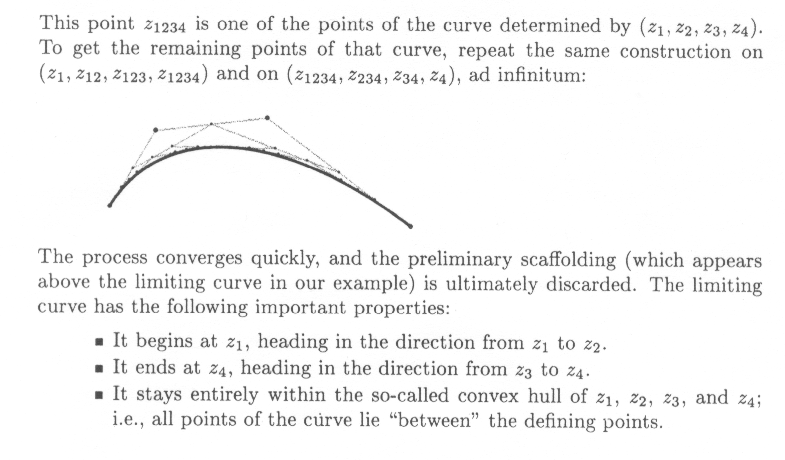
\includegraphics[scale=.3,angle=45]{spline-pic}
\end{examplewithcode}
\item good idea to put this in a float
\end{itemize}
}

\frame[containsverbatim]{
  \frametitle{Text manipulation}
\begin{verbatim}
\usepackage{rotating}
\end{verbatim}
\begin{examplewithcode}
\begin{turn}{30}
Just a line of text
\end{turn}
\end{examplewithcode}
}

\subsection{\LaTeX\ programming}

\frame[containsverbatim]{
  \frametitle{Counters}
\begin{itemize}
\item Use existing counters \n{section}, \n{footnote}, \n{enumi}
\begin{verbatim}
\setcounter{subsection}{3}
\addtocounter{enumii}{-1}
\refstepcounter{footnote}
\arabic{section} \Roman{subsection}
\end{verbatim}
\item Define new counters:
\begin{verbatim}
\newcounter{exercise}[chapter]
\end{verbatim}
\end{itemize}
}

\frame[containsverbatim]{
  \frametitle{Commands}
\begin{examplewithcode}
\newcommand{\IncrByOne}{increased by~$1$}
\dots and $n$~\IncrByOne.
\newcommand{\IncrDecrBy}[2]{#1creased by~$#2$}
\dots and $n$~\IncrDecrBy{de}{5}.
\end{examplewithcode}
(\cs{renewcommand})
}

\frame[containsverbatim]{
  \frametitle{Commands, optional arguments}
\begin{examplewithcode}
\newcommand{\IncrDecrBy}[2][in]{#1creased by~$#2$}
\dots and $x$~\IncrDecrBy{1}.
\dots and $y$~\IncrDecrBy[de]{5}.
\end{examplewithcode}
}

\frame[containsverbatim]{
  \frametitle{New environments}
\begingroup
\begin{examplewithcode}
\renewenvironment{example}%
  {\begin{quote}\tiny\textbf{Example.}}%
  {\end{quote}}
\dots and text.
\begin{example} Blah blah. \end{example}
\end{examplewithcode}
\endgroup
Arguments and optional args as before.
}

\end{document}

\frame[containsverbatim]{
  \frametitle{}
\begin{itemize}
\item
\end{itemize}
}

